\documentclass{article}

% Formatting
\usepackage[utf8]{inputenc}
\usepackage[margin=1in]{geometry}
\usepackage[titletoc,title]{appendix}
\usepackage[spanish]{babel}
\usepackage{amsmath,amsfonts,amssymb,mathtools}
\usepackage{graphicx,float}
\usepackage[ruled,vlined]{algorithm2e}
\usepackage{algorithmic}
\usepackage{minted}
\usemintedstyle{borland}
\usepackage{subcaption}
\usepackage{multicol}
\usepackage{listings}
\usepackage{xcolor}
\usepackage{biblatex}
\addbibresource{ref.bib}
\usepackage{minted}



% Title content
\title{Práctica 12 red neuronal}
\author{Denisse Leyva}
\date{Mayo 18, 2021}

\begin{document}

\maketitle


\section{Introducción}
En esta práctica se vera una demostración básica de aprendizaje de máquina: vamos a reconocer dígitos de imágenes pequeñas en blanco y negro con una red neuronal. El elemento básico de una red neuronal es un perceptrón que esencialmente es un híperplano (una línea si nos limitamos a dos dimensiones) que busca colocarse en la frontera que separa las entradas verdaderas y las entradas falsas. La dimensión $d$ el perceptrón es el largo del vector $x$ que toma como entrada, y su estado interno se representa con otro vector $w$ que contiene sus pesos. Para responder a una salida proporcionada a ello, el perceptrón calcula el producto interno de $x * w$ es decir $\sum_{i=1}^{d}x_{i}=x_{i}w_{i}$ y si esta suma es positiva, la salida del perceptrón es verdad, en otro caso es falso. Para agarrar la onda con los perceptrónes, haremos primero uno más sencillo cuyo jale es identificar si $x > y$ para puntos en dos dimensiones, ya que así es fácil para nosotros visualizar lo que le pasa al perceptrón durante el entrenamiento.

Cada error causa un movimiento en el perceptrón mientras los resultados correctos no le mueven. Las correcciones se hacen gradualmente más pequeñas por la reducción de la tasa de aprendizaje. Terminando el entrenamiento, la línea divisora ya no se mueve. En la fase de prueba, simplemente se clasifican las coordenadas recibidas como verdaderas $(x > y)$ o falsas (en otro caso) \cite{Satu_Elisa_Schaeffer}.

\section{Objetivo}
Estudiar de manera sistemática el desempeño de la red neuronal en términos de su puntaje F (F-score en inglés) para los diez dígitos en función de las tres probabilidades asignadas a la generación de los dígitos (ngb), variando a las tres en un experimento factorial adecuado \cite{Satu_Elisa_Schaeffer}.

\section{Código}
El código base se sacó de Schaeffer \cite{Elisa_Schaeffer}. El código completo se encuentra en el GitHub \cite{Denisse_Leyva}.

\renewcommand{\listingscaption}{Código}
\begin{listing}[H]
  \begin{minted}[linenos,mathescape,texcl]{clojure}
#Se crea el experimento factorial y se guarda en una matriz
fd = fullfact([3, 3, 3])
fd = fd/2
      \end{minted}
  \label{lst:fibo}
  \caption{Creación del experimento factorial.}
\end{listing}

\begin{table}[h!]
\centering
\caption{Tabla experimento factorial.}
 \begin{tabular}{||r r r r||} 
 \hline
 Conteo & n & g & b  \\ [0.5ex] 
 \hline\hline
 1 & 0 & 0 & 0 \\
 \hline
 2 & 0.5 & 0 & 0\\ 
 \hline
 3 & 1 & 0 & 0  \\
 \hline
 4 & 0 & 0.5 & 0 \\
 \hline
 5 & 0.5 & 0.5 & 0 \\
 \hline
 6 & 1 & 0.5 & 0 \\
 \hline
 7 & 0 & 1 & 0 \\
 \hline
 8 & 0.5 & 1 & 0 \\
 \hline
 9 & 1 &  1 & 0  \\
 \hline
 10 & 0 & 0 & 0.5 \\
 \hline
 11 & 0.5 & 0 & 0.5 \\
 \hline
 12 & 1 & 0 & 0.5 \\
 \hline
 13 & 0 & 0.5 & 0.5 \\
 \hline
 14 & 0.5 & 0.5 & 0.5 \\
 \hline
 15 & 1 & 0.5 & 0.5 \\
 \hline
 16 & 0 & 1 & 0.5 \\
 \hline
 17 & 0.5 & 1 & 0.5\\
 \hline
 18 & 1 & 1 & 0.5 \\
 \hline
 19 & 0 & 0 & 1 \\
 \hline
 20 & 0.5 & 0 & 1 \\
 \hline
 21 & 1 & 0 & 1\\
 \hline
 22 & 0 & 0.5 & 1 \\
 \hline
 23 & 0.5 & 0.5 & 1 \\
 \hline
 24 & 1 & 0.5 & 1 \\
 \hline
 25 & 0 & 1 & 1 \\
 \hline
 26 & 0.5 & 1 & 1\\
 \hline
 27 & 1 & 1 & 1\\
 \hline
\end{tabular}
\label{table:1}
\end{table}

\renewcommand{\listingscaption}{Código}
\begin{listing}[H]
  \begin{minted}[linenos,mathescape,texcl]{clojure}
TP = np.diag(cm)
FP = np.sum(cm[:,:-1], axis=0) - TP
FN = np.sum(cm, axis=1) - TP
num_classes = k
TN = []
for i in range(num_classes):
    temp = np.delete(cm, i, 0)    # delete ith row
    temp = np.delete(temp, i, 1)  # delete ith column
    TN.append(sum(sum(temp)))
l = 300
for i in range(num_classes):
    print(TP[i] + FP[i] + FN[i] + TN[i] == l)
precision = TP/(TP+FP)
recall = TP/(TP+FN)    
specificity = TN/(TN+FP)
F_score = 2/ ((1/precision)+(1/recall))
F_score2 = TP / (TP+((FP+FN)/2))    
      \end{minted}
  \label{lst:fibo}
  \caption{Obtención del F score.}
\end{listing}

\section{Resultados}
Como se puede observar existen cuatro combinaciones donde el F score obtuvo los mejores resultados en la combinación "1 0 0", "1 1 0", "0 0 1", "0 1 1", así mismo entre las peores combinaciones que podemos encontrar están la "0.5 0.5 0.5", "1 1 1", "0.5 0 0.5", "0.5 1 0.5". Podemos concluir que para obtener mejores resultados una opción sería mantener a negro y gris altos y otra opción sería mantener blancos altos y negro y gris lo más bajo posible. 

\begin{figure}[H]
\centering
\begin{subfigure}[b]{0.40\linewidth}
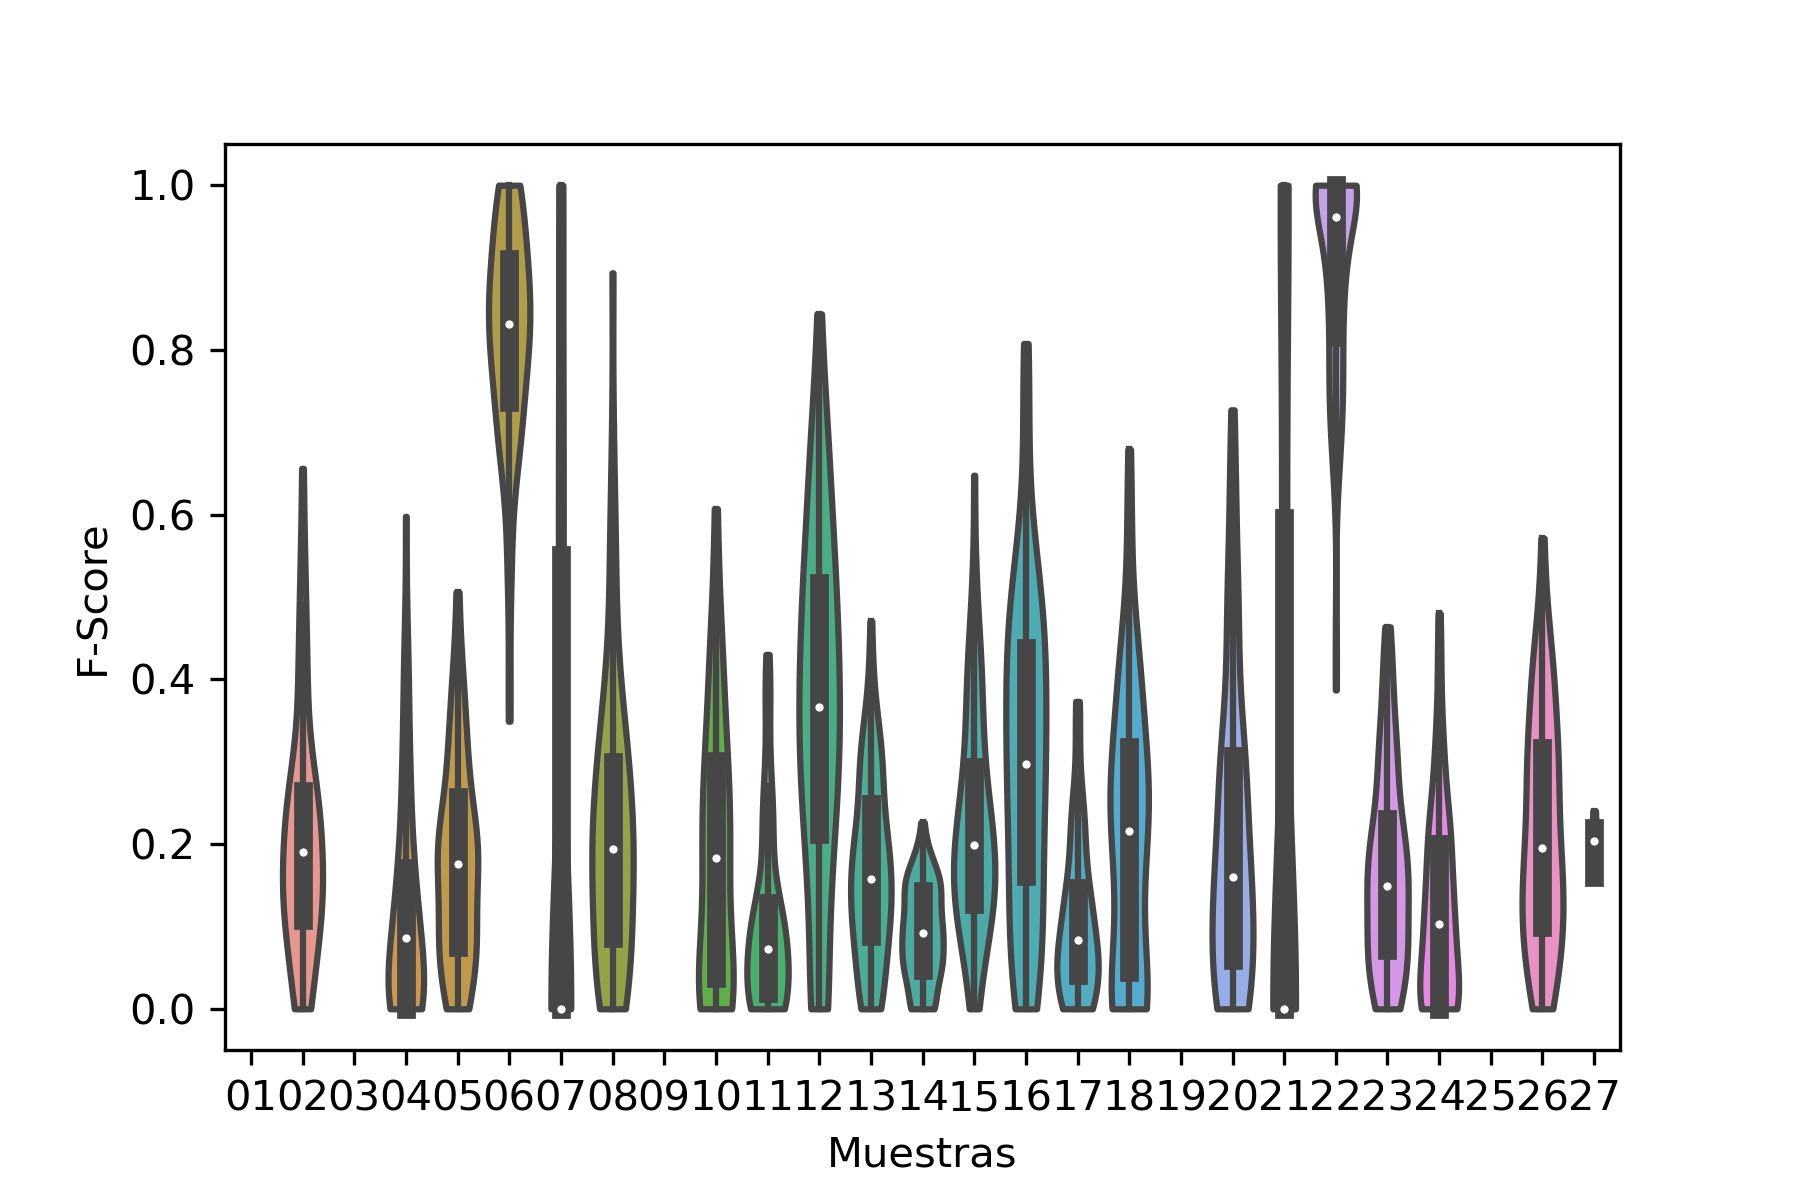
\includegraphics[width=\linewidth]{p11p_2.png}
\caption{resultado del experimento factorial.}
\end{subfigure}
\begin{subfigure}[b]{0.40\linewidth}
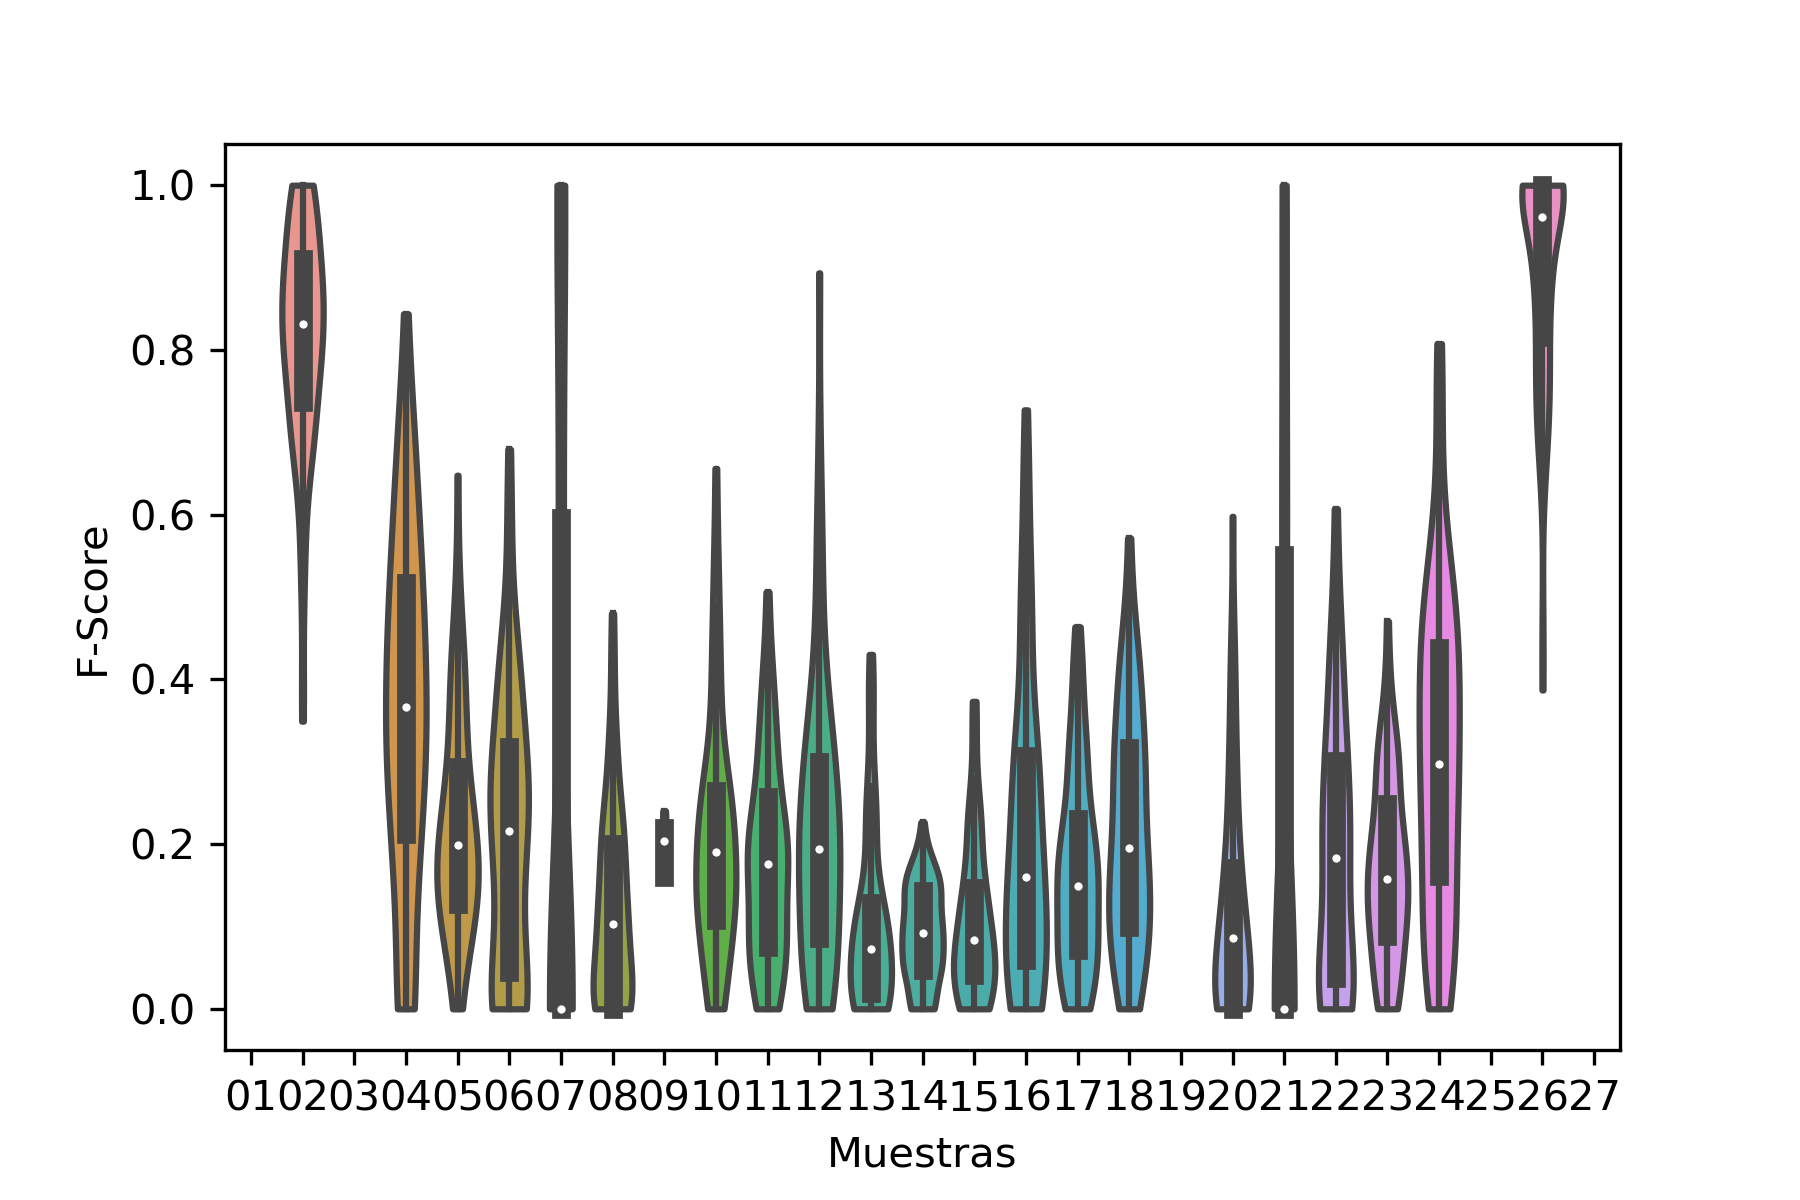
\includegraphics[width=\linewidth]{p11p_3.png}
\caption{resultado del experimetno factorial acomodando $n$ de 1 a 0.}
\end{subfigure}
\caption{Gráficas de resultados obtenidos con el experimento factorial.}
\label{fig:westminster}
\end{figure}

\section{Reto 1}
Como un primer reto, extiende y entrena la red neuronal para que reconozca además por lo menos doce símbolos ASCII adicionales, aumentando la resolución de las imágenes a 5 x 7 de lo original de 3 x 5  (modificando las plantillas de los dígitos acorde a este cambio).

Para este reto se agregó un perceptrón más por la cantidad de dígitos disponibles, y se puede observar en la gráfica de resultados que al momento de tener más dígitos el F score no llega totalmente a 1 como la tarea base. Pero la conclusión es la misma para tener mejores resultados las opciones serian iguales a la tarea base. 

\begin{figure}[H]
\centering
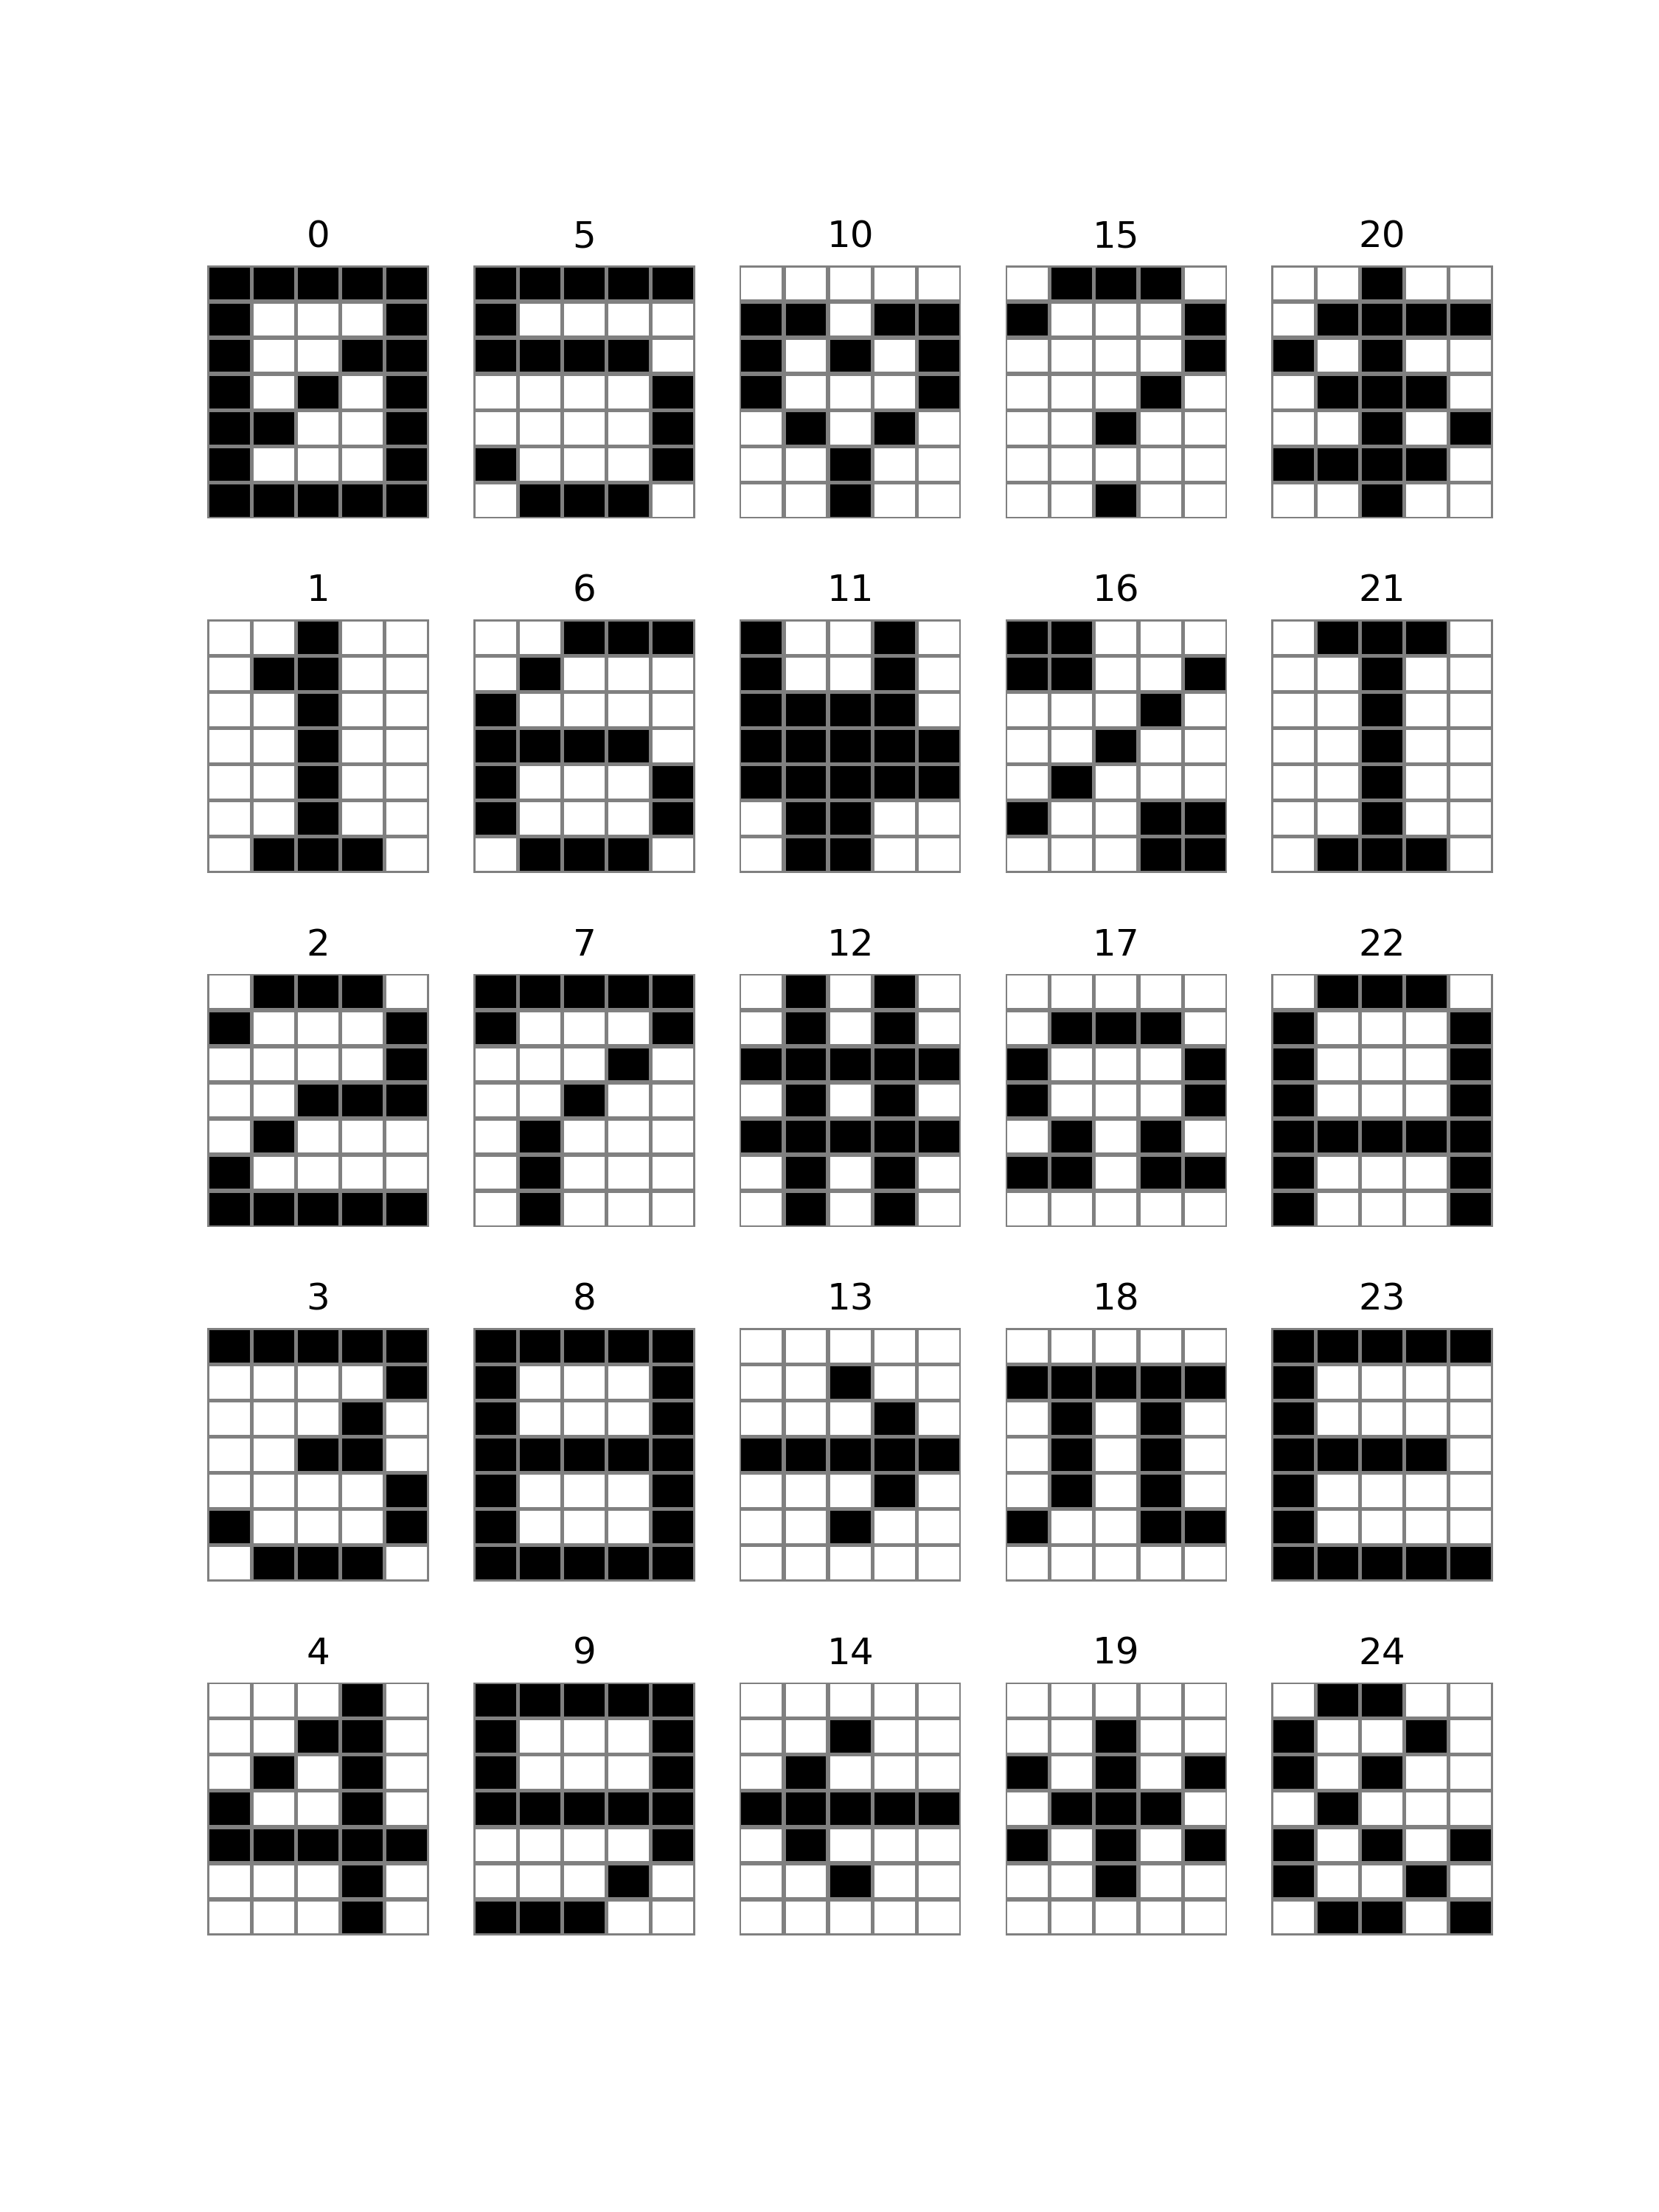
\includegraphics[width=50mm]{p12pg.png}
\caption{\label{fig3} Símbolos ASCII usados para el experimento factorial.}
\end{figure}

\begin{figure}[H]
\centering
\begin{subfigure}[b]{0.40\linewidth}
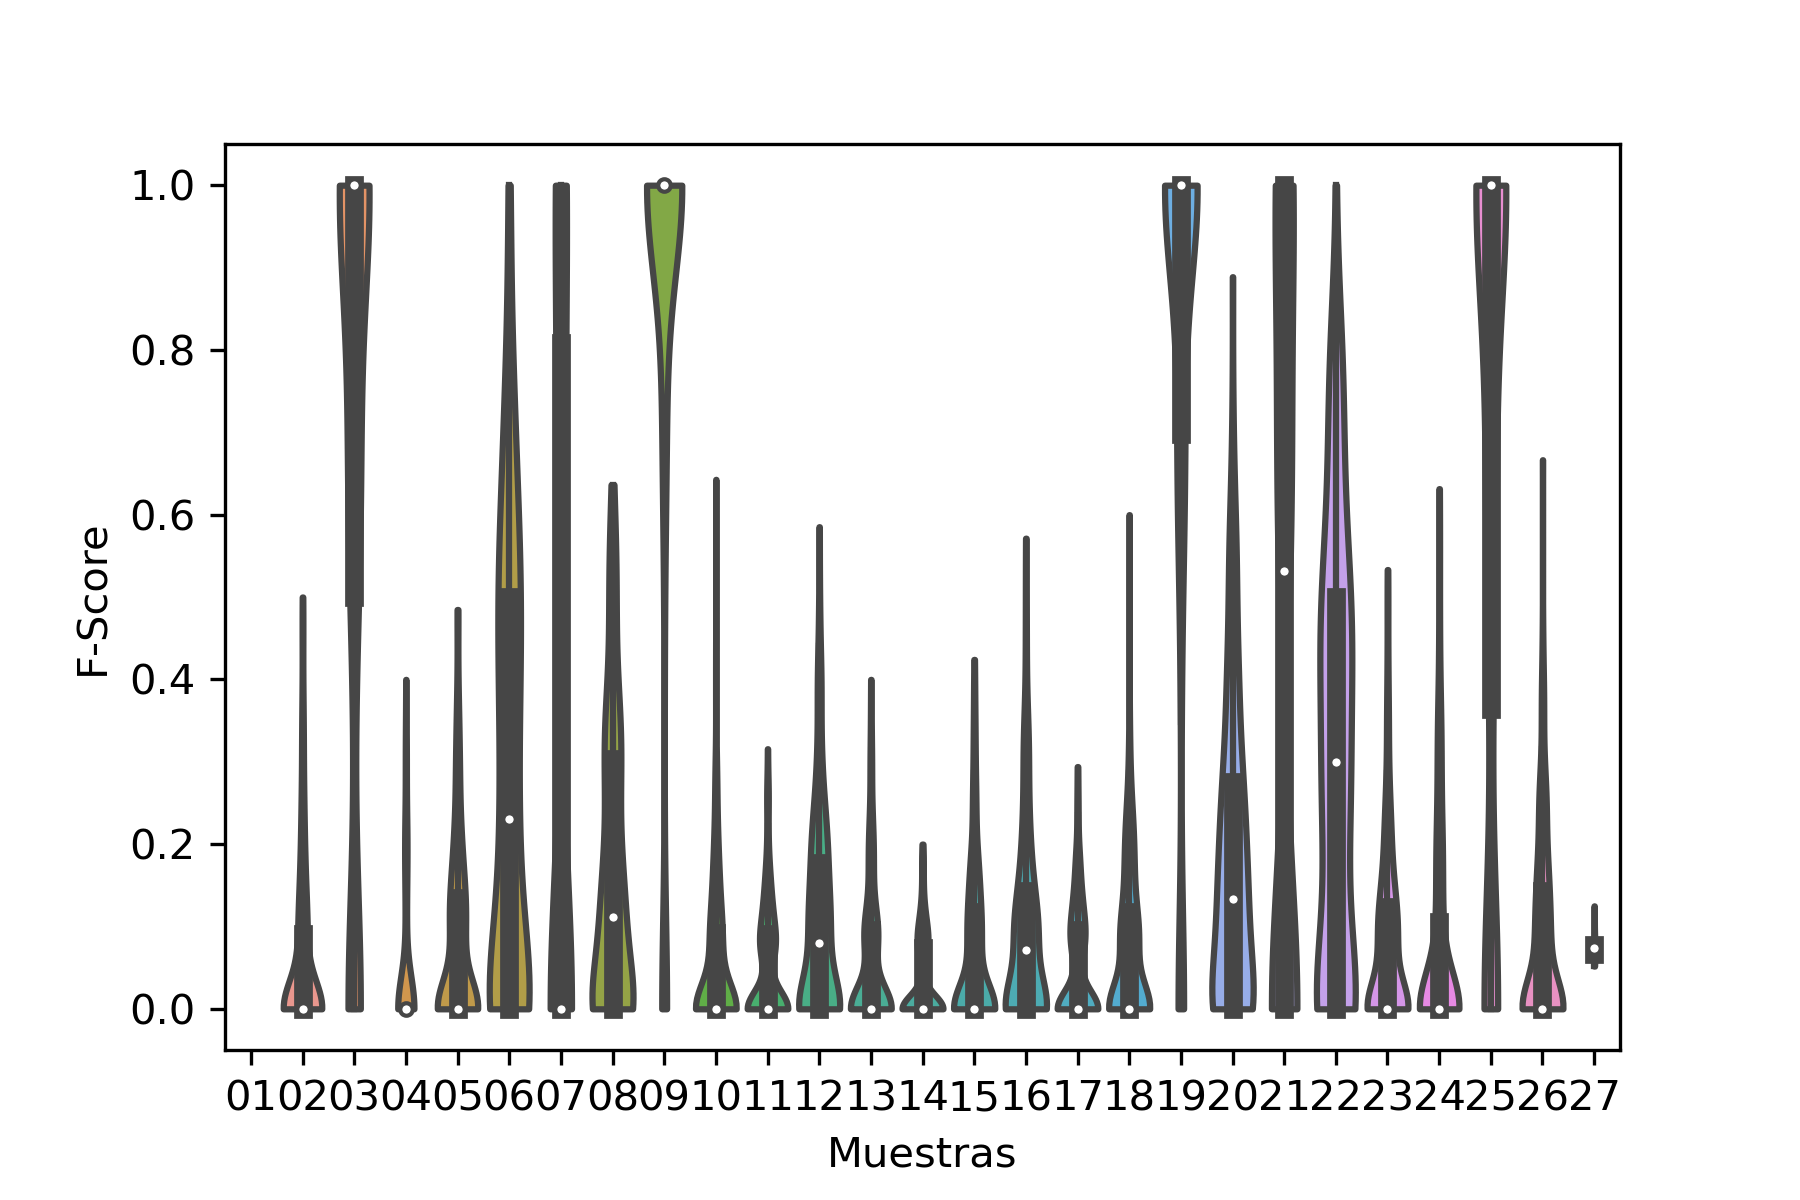
\includegraphics[width=\linewidth]{p11p_r1_2.png}
\caption{resultado del experimento factorial.}
\end{subfigure}
\begin{subfigure}[b]{0.40\linewidth}
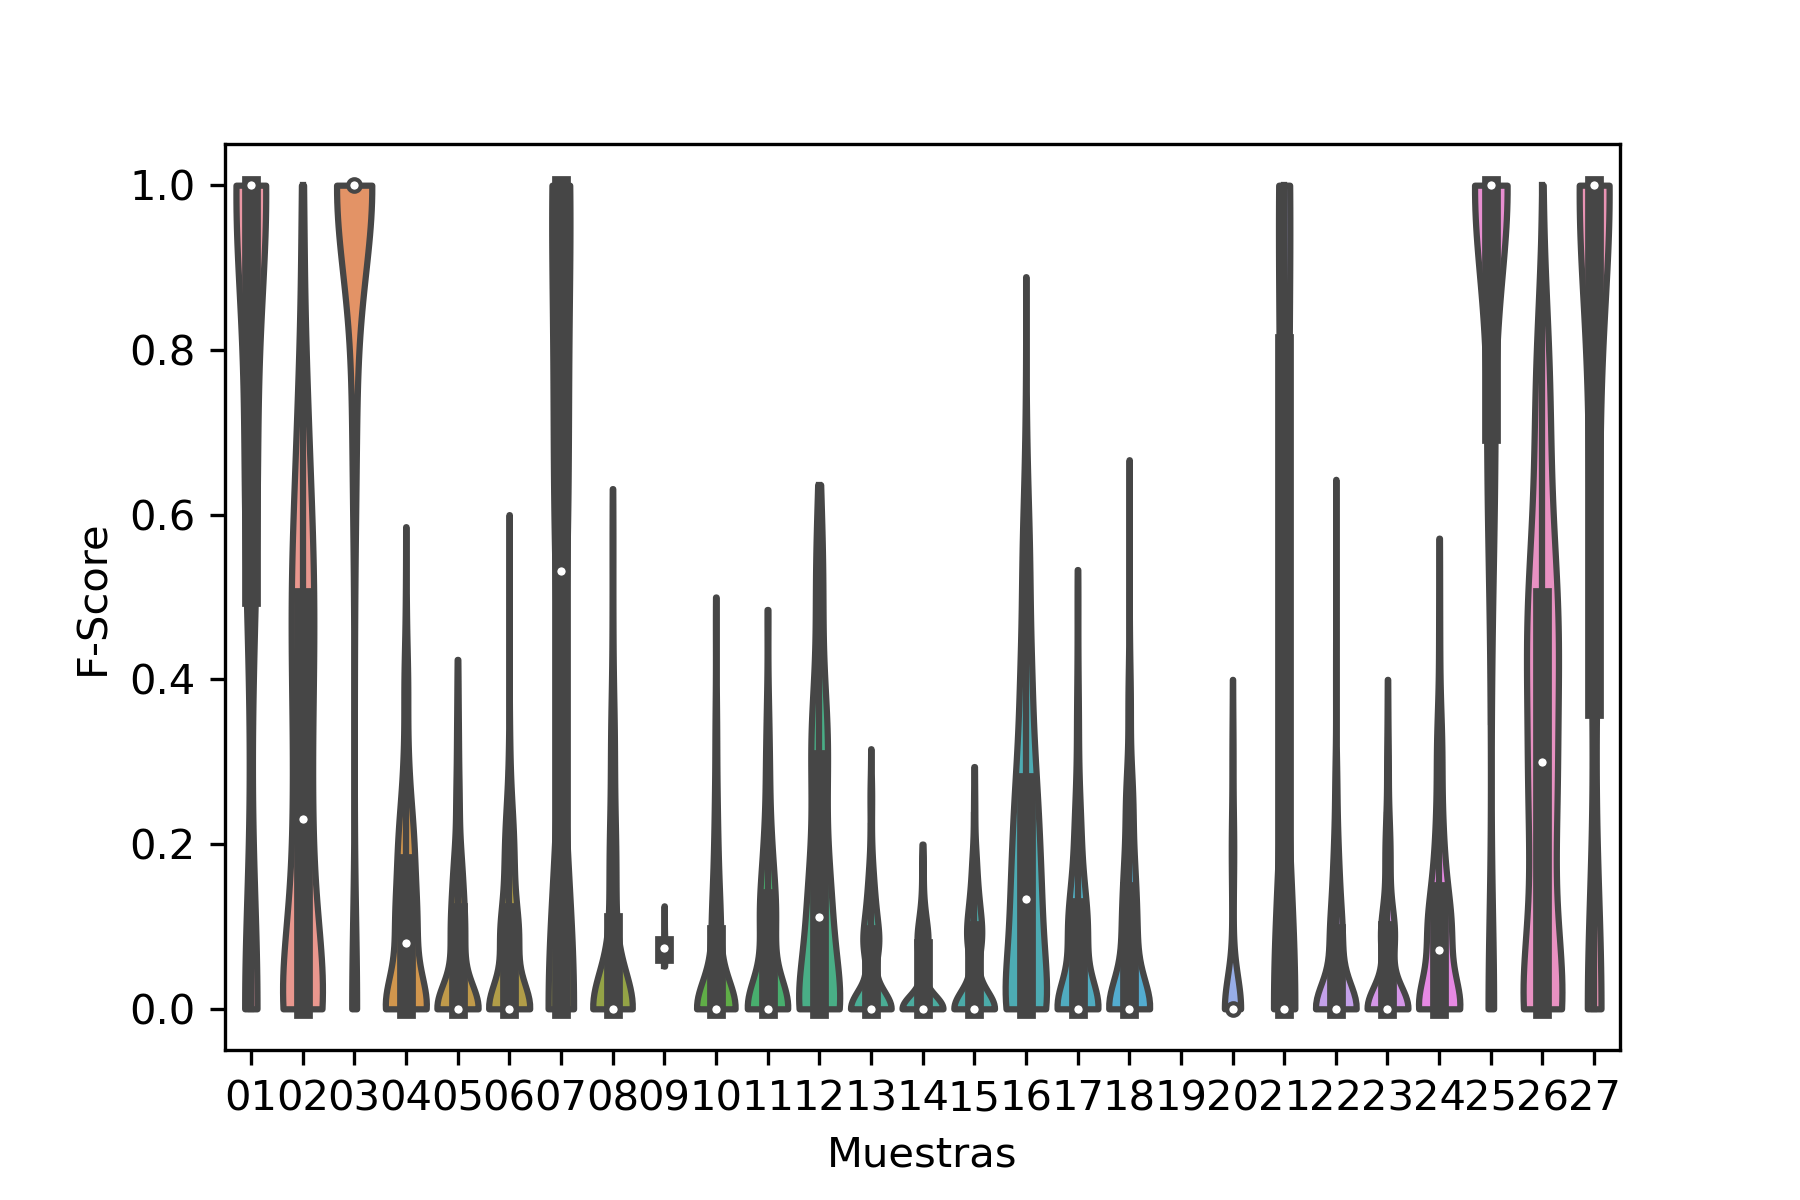
\includegraphics[width=\linewidth]{p11p_r1_3.png}
\caption{resultado del experimetno factorial acomodando $n$ de 1 a 0.}
\end{subfigure}
\caption{Gráficas de resultados obtenidos con el experimento factorial.}
\label{fig:westminster}
\end{figure}


\section{Reto 2}
En este segundo reto se agrega ruido sal-y-pimienta en las entradas para una combinación $ngb$ con la cual la red desempeña bien; este tipo de ruido se genera cambiando con una probabilidad $p_{r}$ los pixeles a blanco o negro (uniformemente al azar entre las dos opciones). Estudia el efecto de $p_{r}$ en el desempeño de la red (no importa si se hace esto con la red de la tarea base o la red extendida del primer reto).

Para este reto se escogió la combinación de "1 1 0" que es de las mejores combinaciones en la tarea base, a esta combinación se le agrego ruido sal y pimienta que va con un porcentaje de probabilidad de 10\% del 0 al 100.

\renewcommand{\listingscaption}{Código}
\begin{listing}[H]
  \begin{minted}[linenos,mathescape,texcl]{clojure}
 for t in range(5000): # entrenamiento
    d = randint(0, tope)
    pixeles = abs(1 * (np.random.rand(dim) < modelos.iloc[d]) - (np.random.uniform(size = dim)<pr))
    correcto = '{0:04b}'.format(d)
    for i in range(n):
        w = neuronas[i, :]
        deseada = int(correcto[i]) # 0 o 1
        resultado = sum(w * pixeles) >= 0
        if deseada != resultado: 
            ajuste = tasa * (1 * deseada - 1 * resultado)
            tasa = tranqui * tasa 
            neuronas[i, :] = w + ajuste * pixeles
      \end{minted}
  \label{lst:fibo}
  \caption{Para agregar ruido sal y pimienta.}
\end{listing}

\begin{figure}[H]
\centering
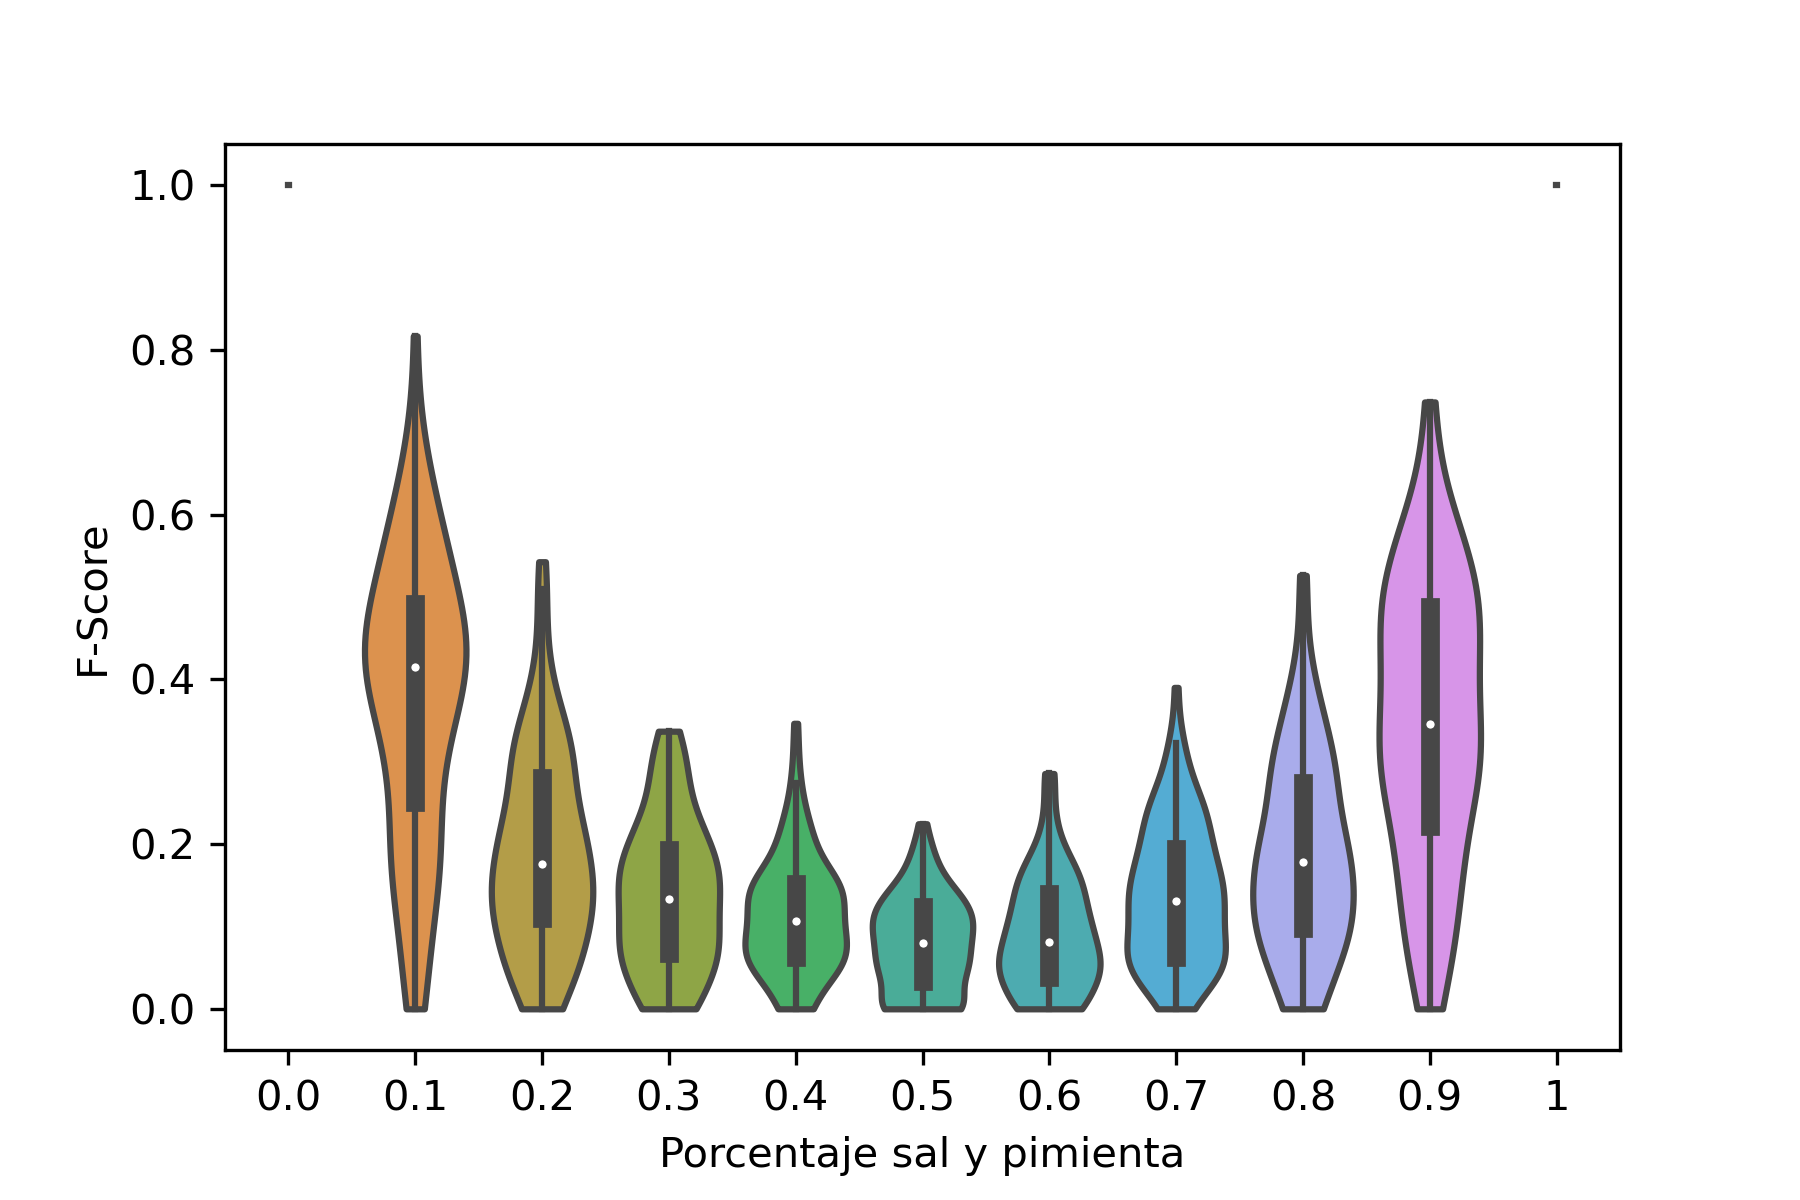
\includegraphics[width=80mm]{p11p_r2_1.png}
\caption{\label{fig3} Gráfica mostrando el porcentaje del ruido.}
\end{figure}

\printbibliography
\end{document}
